\documentclass[11pt,a4paper]{amsart}

%\usepackage{amssymb, amsmath, amsthm, latexsym}
%\usepackage[alphabetic]{amsrefs}
%\usepackage{calrsfs}
%\usepackage{graphicx}
\usepackage{tikz}
\usepackage{float}




\def\R{{\mathbb R}}
\def\Q{{\mathbb Q}}
\def\Z{{\mathbb Z}}
\def\C{{\mathbb C}}
\def\S{{\mathbb S}}
\def\N{{\mathbb N}}
\def\H{{\mathbb H}}
\def\RP{{\mathbb {RP}}}
\def\p{\partial}
\def\O{\Omega}
\def\pO{{\partial\Omega}}
\def\bO{\overline\Omega}
\def\a{\alpha}
\def\b{\beta}
\def\g{\gamma}
\def\G{\Gamma}
\def\d{\delta}
\def\D{\Delta}
\def\e{\epsilon}
\def\r{\rho}
\def\t{\tau}
\def\l{\lambda}
\def\L{\Lambda}
\def\k{\kappa}
\def\s{\sigma}
\def\th{\theta}
\def\o{\omega}
\def\z{\zeta}
\def\n{\nabla}
\def\T{{\mathcal T}}
\def\X{{\mathcal X}}
\def\area{\mathrm{area}}
\def\dist{\mathrm{\rm dist}}
\def\diag{\mathrm{diag}}
\def\spt{\mathrm{spt\,}}
\def\diam{\mathrm{diam\,}}
\def\dim{\mathrm{dim\,}}
\def\graph{\mathrm{graph\,}}
\def\interior{\mathrm{interior\,}}
\def\diag{\mathrm{diag\,}}
\def\Image{\mathrm{Image}\,}
\def\osc{\mathop{\text{\rm osc}}}


\def\ra{\rightarrow}
\def\rai{\rightarrow\infty}

\overfullrule0pt \hoffset=0cm
\parskip=4pt
\parindent=0pt
\baselineskip=20pt

\begin{document}

\thispagestyle{empty}
\begin{center}
\huge
\vspace*{1.0in} MATH2320/3116/6110
\\\vspace{0.5in} \textsc{Assignment 3}
\normalsize
\\\vspace{0.5in} \textsc{By}
\\\vspace{0.1in} \textsc{Zeming Wang}
\\\vspace{0.1in} \textsc{u6114134}
\normalsize
\\\vspace{0.5in} \textsc{Lecture: John Urbas}
\\\vspace{0.1in} \textsc{Tutor: Sophie Chen}
\\\vspace{0.1in} \textsc{Tutorial: Wednesday 5-6 pm}
\normalsize
\\\vspace{0.5in} \textsc{Due: 23 April 2018}
\end{center}

\newpage
\setcounter{page}{1}


%All questions are of equal value.

%\bigskip



{\bf 1.} [8+4+4= 16 points]

(a) Two metrics $d_1$ and $d_2$ are said to be {\it equivalent} if every set that is open
in $(X,d_1)$ is open in $(X,d_2)$ and vice versa.

Prove that two metrics $d_1$ and $d_2$ are equivalent if and only if for every $x\in X$
and every $\varepsilon>0$ there is a $\delta>0$ such that
$$ B_\d^{d_1}(x) \subset B_\e^{d_2}(x)
\qquad\mbox{and}\qquad
B_\d^{d_2}(x) \subset B_\e^{d_1}(x). $$


\begin{proof}
Suppose $d_1$ and $d_2$ are equivalent.
Since $B_\e^{d_2}(x)$ is open in $(X, d_2)$, it is open in $(X, d_1)$.
Therefore there exists a $\d>0$ such that $ B_\d^{d_1}(x) \subset B_\e^{d_2}(x)$.
Symmetrically, since $B_\e^{d_1}(x)$ is open in $(X, d_1)$, it is open in $(X, d_2)$.
Therefore there exists a $\d>0$ such that $ B_\d^{d_2}(x) \subset B_\e^{d_1}(x)$. \\

Suppose  for every $x\in X$ and every $\varepsilon>0$ there is a $\delta>0$ such that
$ B_\d^{d_1}(x) \subset B_\e^{d_2}(x) $ and $B_\d^{d_2}(x) \subset B_\e^{d_1}(x)$.
If $A$ is open in $(X, d_1)$, by definition, $\forall x \in A$, $\exists \e>0$ such that
$B_{\e}^{d_1}(x) \subset A$; and by our assumption, $\exists\d>0$ such that
$B_\d^{d_2}(x) \subset B_\e^{d_1}(x)$. Thus $B_\d^{d_2}(x) \subset A$.
This holds for all $x\in A$, which implies $A$ is open in $(X, d_2)$.
Symmetrically, we can prove if $A$ is open in $(X,d_2)$, it is open in $(X,d_1)$.
Hence, $d_1$ and $d_2$ are equivalent.
\end{proof}

\medskip

(b) Show that the following metrics on $\R^n$ are equivalent:

\begin{align*}
d_1(x,y) &= \sum_{i=1}^n |x_i-y_i| \\
d_2(x,y) &= \left[\sum_{i=1}^n (x_i-y_i)^2\right]^{1/2} \\
d_3(x,y) &= \max_{i\in\{1,\dots,n\}} |x_i-y_i|.
\end{align*}


\begin{proof}
For $p$-norms on $\R^n$, we have $\|x\|_p \ge \|x\|_q$ if $1 \le p \le q \le \infty$.\\

Therefore, we have
$$ d_1(x,y) \ge d_2(x,y) \ge d_3(x,y)$$
and thus
$$B_{\e}^{d_1}(x) \subset B_{\e}^{d_2}(x) \subset B_{\e}^{d_3}(x)$$

For given $B_{\e}^{d_1}(x)$, take $\d = \dfrac{\e}{\sqrt{n}}$.

By Cauchy-Schwartz inequality, $d_2(x,y) < \d$ implies

\begin{align*}
    d_1(x,y) = \sum_{i=1}^n |x_i-y_i|\cdot 1
      &\le \left[\sum_{i=1}^n (x_i-y_i)^2\right]^{1/2} \cdot
            \left[\sum_{i=1}^{n}1^2\right]^{1/2} \\
      &= \sqrt{n}\cdot d_2(x,y) < \sqrt{n} \cdot \frac{\e}{\sqrt{n}} = \e
\end{align*}

Therefore $B_\d^{d_2}(x) \subset B_\e^{d_1}(x)$.
Together with $B_{\d=\e}^{d_1}(x) \subset B_{\e}^{d_2}(x)$, this proves
$d_1$ and $d_2$ are equivalent. \\

Given $B_{\e}^{d_1}(x)$, take $\d = \dfrac{\e}{n}$. Then $d_3(x,y)<\delta$ implies
\begin{align*}
    d_1(x,y) = \sum_{i=1}^n |x_i-y_i|
             &\le n \cdot \max_{i} |x_i-y_i| \\
             &= n\cdot d_3(x,y) < n \cdot \frac{\e}{n} = \e
\end{align*}

Therefore $B_\d^{d_3}(x) \subset B_\e^{d_1}(x)$. This shows
$d_1$ and $d_3$ are equivalent. \\

Therefore, $d_1, d_2, d_3$ are all equivalent.
\end{proof}
\medskip

(c) The vector space of continuous functions on $[0,1]$ can be given the two metrics
$$ d_\infty(f,g) = \sup_{x\in[0,1]} |f(x)-g(x)| $$
and
$$ d_2(f,g) = \left( \int_0^1 |f(x)-g(x)|^2\, dx\right)^{1/2}. $$

Are these two metrics equivalent? Provide a reason for your answer.

\begin{proof}[Solution.]
  No. Consider $g(x)=0$ and $f_n(x)$ is the function below:

  \begin{figure}[H]
    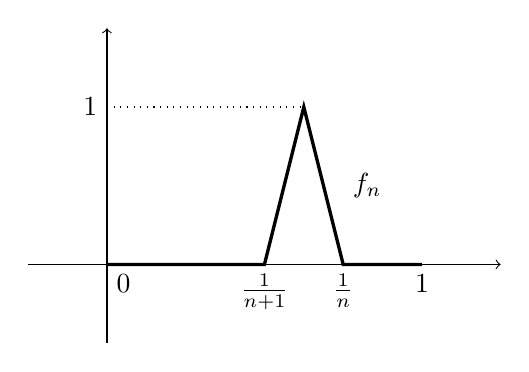
\begin{tikzpicture}
      \draw [->] (-1, 0) -- (5, 0);
      \draw [->] (0, -1) -- (0, 3);
      \node [below right] at (0,0) {$0$};
      \node [below] at (4,0) {$1$};
      \node [below] at (2,0) {$\frac{1}{n+1}$};
      \node [below] at (3,0) {$\frac{1}{n}$};
      \draw [very thick] (0,0) -- (2,0) -- (2.5,2) -- (3,0) -- (4,0);
      \draw [dotted] (0,2) -- (2.5,2);
      \node [left] at (0,2) {$1$};
      \node [right] at (3,1) {$f_n$};
    \end{tikzpicture}
    % \caption{Figure 1}
    \label{fig_1}
  \end{figure}

  It is easy to see that $d_{\infty}(f_n, g) = 1$ for all $n$; and as $n\to\infty$,
  $$ d_2(f_n,g)  \le \sqrt{ \int_0^1 (f_n(x)-g(x)) dx } \to 0. $$

  Therefore, $\forall \d >0$, $\exists N \in\N$, such that $\forall n>N$, we have
  $f_n \in B_{\d}^{d_2}(g)$. But $f_n \not\in B_{\e}^{d_{\infty}}(g)$ if
  $0 < \e < 1$. This is a violation for the necessary and sufficent condition
  for $d_\infty$ and $d_2$ to be equivalent.
\end{proof}

\bigskip


{\bf 2.} [4+4+4=12 points]

A set $A$ in a metric space $(X,d)$ is said to be {\it dense} in $X$ if its closure is $X$.

(a) Let $f$ be a continuous function from a metric space $(X,d)$ into a metric space
$(Y,\rho)$. Prove that if $E$ is dense in $X$, then $f(E)$ is dense in $f(X)$. \hfil $(*)$

\begin{proof}
  To show $f(E)$ is dense in $f(X)$,  we need to show every point in $f(X)$ is
  either a point in $f(E)$ or a limit point of $f(E)$.

  Suppose $y \in f(X)$. Then there exists $x \in X$ such that $f(x) = y$.
  Since $E$ is dense in $X$, $x$ is either (1) a point in $E$,  or
  (2) a limit point of $E$.

  \begin{enumerate}
    \item[(1)] If $x \in E$, then $f(x) \in f(E)$.
    \item[(2)] If $x$ is a limit point of $E$,
                $\exists (x_n)\subset E$ such that $x_n \to x$.
                Then by continuity of $f$, we have $f(x_n) \to f(x)$.
                Since $f(x_n)\subset f(E)$, $f(x)$ is a limit point of $f(E)$.
  \end{enumerate}

  By (1) and (2), $y=f(x)$ is either a point in $f(E)$ or a limit point of $f(E)$,
  which proves $f(E)$ is dense in $f(X)$.
\end{proof}
\medskip

(b) If $g$ is another continuous function from $(X,d)$ into $(Y,\rho)$ such that $f(z)=g(z)$
for all $z\in E$ where $E$ is dense in $X$, show that $f(x)=g(x)$ for all $x\in X$.
[In other words, a continuous function is completely determined by its values on a dense subset
of $X$.]

\begin{proof}
  $E$ is dense in $X$, so $\forall x\in X$, either $x\in E$, or $x$ is a limit point of $E$.

  \begin{enumerate}
    \item If $x\in E$, $f(x)=g(x)$ by assumption and we are done.
    \item If $x$ is a limit point of $E$, $\exists (x_n)\subset E$ such that $x_n\to x$.
          Since $f$ and $g$ are both continuous on $X$, we have $\lim_{n\to\infty} f(x_n) = f(x)$, and
          $\lim_{n\to\infty} g(x_n) = g(x)$.
          Note $f(x_n) = g(x_n)$ for all $n$.
          Therefore it must be $f(x) = g(x)$.
  \end{enumerate}

  Hence, $f(x)=g(x)$ for all $x\in X$.
\end{proof}
\medskip

(c) Prove or provide a counterexample: If $f:E\rightarrow Y$ is continuous on a dense subset
$E$ of a metric space $X$, then there is a continuous function $\bar f:X\rightarrow Y$
such that $\bar f(z)=f(z)$ for all $z\in E$.

\begin{proof}[Solution.]
  The statement is not true.
  For example, let $f: \Q \to \R$ be
  $$f(x) = \frac{1}{x-\pi}$$
  $f$ is continuous on $\Q$ because whenever $(q_n) \to q \in \Q$, we have $f(q_n)\to f(q)$.
  But $f$ fails to be continuous when extended to $\R$ (it is discontinuous at $\pi$),
  though $\Q$ is dense in $\R$. In fact, there is no $\bar{f}$ which is continuous on $\R$
  and $\bar{f}(x) = f(x)$ for all $x\in\Q$.
\end{proof}
\medskip


% $(*)$ The meaning of this may appear to be ambiguous, but it is not. According to the definition given above,
% $f(E)$ is dense in $f(X)$ means that $\overline{f(E)}=f(X)$ where the closure is taken
% in the metric space $(f(X),d)$. Another way to say this
% is that if $y\in f(X)$, then there is a sequence $(y_n)$ in $f(E)$ such that $\rho(y_n,y)
% \rightarrow 0$.
%
% If $\overline{f(E)}$ is interpreted as the closure in $(Y,d)$, then it may happen that
% $\overline{f(E)}\supset f(X)$ with strict inclusion
% (try to construct such an example).

\bigskip


{\bf 3.} [4+4+4+5=17 points]

Let $r\in(0,1)$, and let $C[0,r]$ denote the space of continuous real valued functions on $[0,r]$ equipped
with the supremum metric
$$ d(f,g)=\sup_{x\in[0,r]}|f(x)-g(x)|.  $$
You may assume that $(C[0,r],d)$ is complete ---
this will be proved in lectures.

(a) Let $a\in\R$. Show that the mapping $T:C[0,r]\ra C[0,r]$ defined  by
$$ (Tf)(x) = a + \int_0^x f(t)\, dt $$
is a contraction on $(C[0,r],d)$.

\begin{proof}
  \begin{align*}
    d(Tf, Tg) &= \sup_{x\in[0,r]} \left\rvert \int_0^x f(t) dt - \int_0^x g(t) dt \right\rvert \\
      &= \sup_{x\in[0,r]} \left\rvert \int_0^x (f(t) -g(t)) dt \right\rvert \\
      &\le \sup_{x\in[0,r]}  \int_0^x |f(t) -g(t)| dt  \\
      &\le \int_0^r |f(t) -g(t)| dt \\
      &\le \int_0^r \sup_{x}|f(x) -g(x)| dt \\
      &= \sup_{x}|f(x) -g(x)| \int_0^r dt \\
      &= r \cdot d(f,g)
  \end{align*}
  where $r\in(0,1)$. Therefore $T$ is a contraction.
\end{proof}
\medskip

(b) Does $T$ have a fixed point? If so, is it unique? Give reasons for your answers.
	If you answered yes to both, what is the fixed point?

  \begin{proof}[Solution.]
    Yes. $(C[0,r],d)$ is complete, and $T$ is a contraction.
    By Banach Fixed-Point Theorem, there exists a fixed point, and it is unique. \\

    Suppose $f(x)$ is the fixed point, i.e.
    $$ f(x) = a + \int_0^x f(t)\, dt $$

    Then by the Fundamental Theorem of Calculus,
    $$ f'(x) = f(x) $$

    It is easy to guess $f(x) = e^x$, which is the fixed point.
  \end{proof}

\medskip

(c) Now consider the case $r=1$. Let $T$ be defined as above.
Is $T$ a contraction on $(C[0,1],d)$? Prove your answer.
Does $T$ have a fixed point? Explain.

\begin{proof}[Solution.]
  If $r=1$, $T$ is no longer a contraction.

  To show a counterexample,
  let $f(x)=2, g(x)=1$. Then $d(f,g) = 1$, and
  $$ d(Tf, Tg) = \sup_{x\in[0,1]} \left\rvert \int_0^x 1\ dt \right\rvert = \sup_{x\in[0,1]} |x| = 1 $$
  Therefore $d(Tf, Tg) = d(f,g)$ is not a contraction. \\

  But $T$ still has a fixed point. $f(x) = e^x,\ x\in[0,1]$ is still a fixed point.
\end{proof}
\medskip

(d) Let $C^1[0,1]$ be the set of all functions in $C[0,1]$ that have a continuous derivative on $[0,1]$ (we take one sided derivatives at the endpoints). We equip $C[0,1]$ with the usual supremum metric. Then $C^1[0,1]$ is a subspace of $C[0,1]$.
Define $\Phi:C^1[0,1]\ra C[0,1]$ by $\Phi(f)=f'$. Is $\Phi$ continuous? Prove your answer.

\begin{proof}[Solution.]
  $\Phi$ is not necessarily continuous.

  Consider $f_n \in C[0,1]$ given below:

  \begin{figure}[H]
    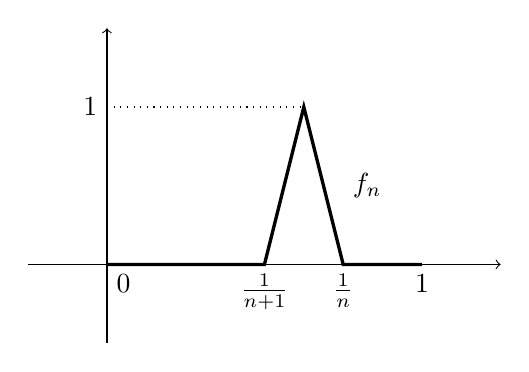
\begin{tikzpicture}
      \draw [->] (-1, 0) -- (5, 0);
      \draw [->] (0, -1) -- (0, 3);
      \node [below right] at (0,0) {$0$};
      \node [below] at (4,0) {$1$};
      \node [below] at (2,0) {$\frac{1}{n+1}$};
      \node [below] at (3,0) {$\frac{1}{n}$};
      \draw [very thick] (0,0) -- (2,0) -- (2.5,2) -- (3,0) -- (4,0);
      \draw [dotted] (0,2) -- (2.5,2);
      \node [left] at (0,2) {$1$};
      \node [right] at (3,1) {$f_n$};
    \end{tikzpicture}
    % \caption{Figure 1}
    \label{fig_2}
  \end{figure}

  Let $$ F_n(x) = \int_0^x f_n(t)\ dt $$
  Then $F_n \in C^1[0,1]$ and $\Phi(F_n) = f_n$.
  And as $n\to\infty$, $F_n(x) \to 0$ (the area below the curve diminishes to $0$).

  Let $G(x)=0$ and $g(x) = \Phi(G(x)) = 0$. Then
  $d(F_n, G) \to 0$ as $n\to\infty$.
  But $d(f_n, g) = \sup |f_n(x) - 0| = 1$ for all $n$.

  Therefore, $\Phi$ fails to be continuous at such $F_n$.
\end{proof}

\end{document}
